\chapter{Analysis}
\section{Abstract}
As I am an A Level Maths (with mechanics) and Physics student, I have studied the topics of projectile motion and radioactive decay. I myself found these topics to be difficult as did many other of my peers. The current method of practising mathematics and physics questions is to attempt problems from a course textbook. As there are many questions for the student to try, they can seem repetitive or boring causing the student to be more likely to stop. This can be solved by providing a range of questions to provide variety. The majority of problems are provided with no diagram, so the student has to interpret the text and potentially draw their own diagram. While this type of question is likely to come up in the exam, when the student is first learning the topic, it is important that they understand the topic fully before attempting harder, exam style questions. This can be solved by providing diagrams for the student. This allows the question text to be represented visually which make the problem easier to understand, and it will allow the student to relate the question to the underlying concepts that they are learning.

This software will be an easy to use platform. It will generate questions from the projectile motion and radioactive decay topics, and will draw graphs to go with these. The main aim of the software is to be a learning tool, to help students understand the basics of these topics.
\section{Features of the proposed solution that can be solved using computational methods}
\subsection{Random nature of questions}
The questions will be randomly generated. The base question will be stored so that there are elements within it that can be changed. This allows a loop to be created, which will produce \textit{n} amount of questions, with the elements being changed to a random number from a specified range. The generated elements can then be used to create the diagram or graph, by putting these elements into the diagram generation function.
\subsection{Answer Verification}
The number of significant figures in the student will not matter. If the student's answer is the same as the calculated answer to any number of significant figures it will be marked as correct. Computationally, this can be implemented by using built in \textbf{round} functions, meaning that the mathematics behind this does not have to be coded from scratch. This will be faster than if this was implemented non-computationally.
\subsection{Generation of diagrams}
For both projectile motion and radioactive decay, graphs can be generated using an iterative method. This works by supplying an equation with a variable that can be incremented. This is usually time \textit{t}. The equation then outputs a value that plotted as the y coordinate on a graph, with the x coordinate being the time value inputted into the equation. This solution will enable graphs of projectile motion and radioactive decay to be quickly generated for display.
\section{Stakeholders}
Students studying A Level physics are the main target users of this program. It will offer an unlimited supply of questions to practice outside of the textbook. The questions will be provided with a graph or diagram which could make the question seem easier to some. This is intended, as the program is meant to aid understanding of the fundamentals of these topics. 
A Level physics teachers are another target group. They will be able to use this tool in initial lessons to demonstrate how to answer these type of questions. The generated graph will enable easy explanation of the question, and will save time for the teacher. Once the basics have been covered, teachers could task students to complete questions on the application.
\clearpage
\section{Existing Solutions}
\begin{figure}[h]
	\centering
	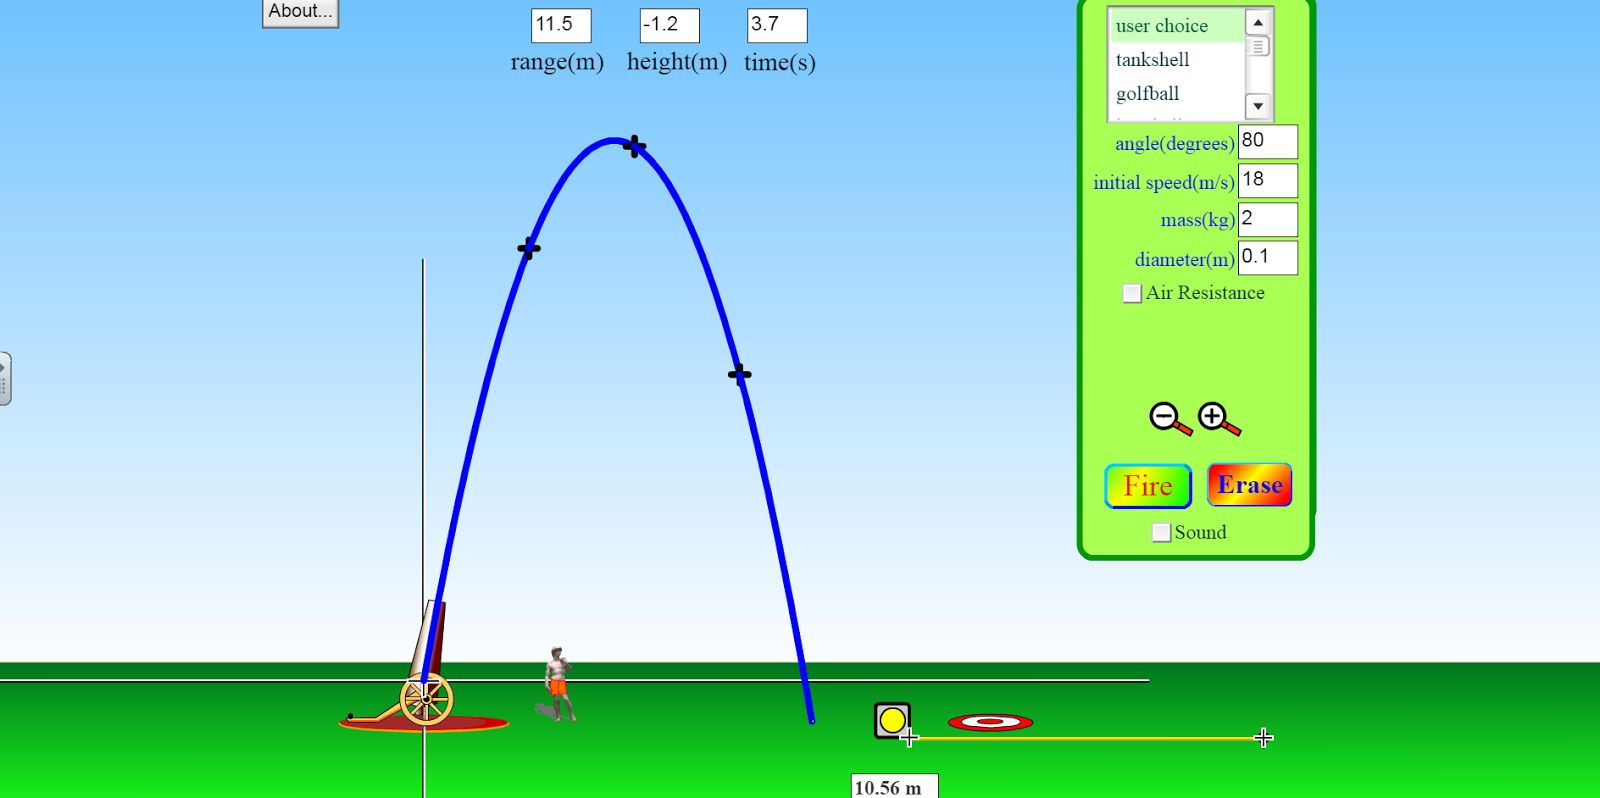
\includegraphics[width=\textwidth,height=\textheight,keepaspectratio]{Analysis-000}
	\caption{PHET Interactive projectile motion simulator \protect\cite{PHET}
\end{figure}
This software allows the user to 

	